\chapter{Background} \label{chap:background}
% -------------------------
%% QUOTE
\vspace*{\fill}
\epigraph{The more we learn about the world, and the deeper our learning, the more conscious, specific, and articulate will be our knowledge of what we do not know, our knowledge of our ignorance.\\ For this, indeed, is the main source of our ignorance — the fact that\\ \textbf{our knowledge can be only finite, while our ignorance must necessarily be infinite.}}%
{\textit{Conjectures and Refutations (1963)}\\ \textsc{Karl Popper}}
\clearpage{\thispagestyle{empty}\cleardoublepage}
%%
%% Body of the chapter
%%%%%%%%%%%%%%%%%%%%%%
\section{Nanoparticles and their applications}
If we assumed a range for all the sizes colloids could assume, Nanoparticles would be at the smaller end of it \citep{Goodwin2009}. The different industries have, in the last decade or two, found significant applications for nanoparticles in manufacturing products with special characteristics. In all these applications, the small size of nanoparticles is exploited for development of new materials, tools and devices. Generally speaking, ``nanoparticles" are particles whose dimensions (at least one dimension) are smaller than 100 nm. At these lengths, special electronic, thermal, mechanical and chemical properties appear (such as greater surface area per volume, higher reactivity with other molecules), the application of which can enable a plethora of new solutions. Figure \ref{cht:NPsurfaceVolume} shows surface area to volume ratio of the same volume of materials in ranges of millimeter, micrometer and nanometer. As illustrated by \cite{Amanullah2009}, conversion of a particle from the millimeter scale to the nanometer scale will multiply its area to volume ratio a million fold. 
\begin{figure}[h]
    \centering
    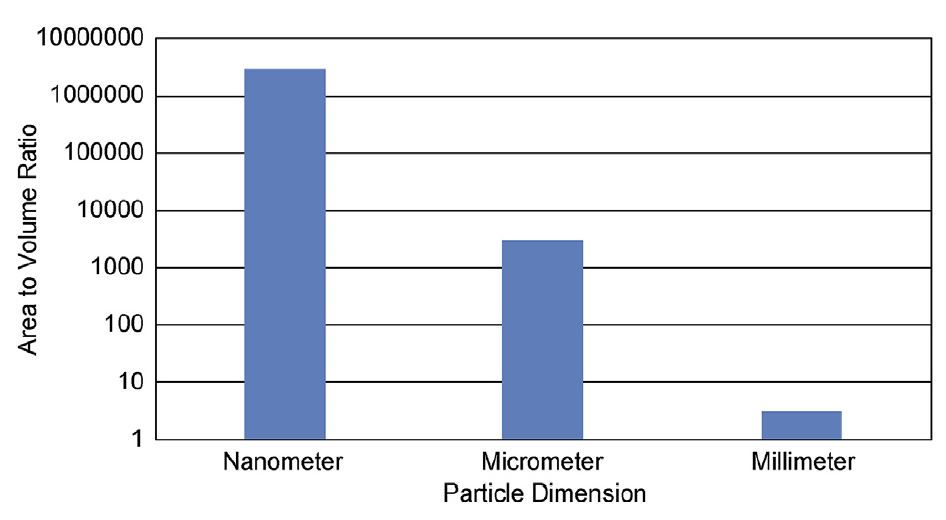
\includegraphics[width=\textwidth]{img/cht/NPsurfaceVolume.png}
    \caption{Surface area to volume ratio of the same volume of materials (adapted from \cite{Amanullah2009})}
    \label{cht:NPsurfaceVolume}
\end{figure}

\cite{Fakoya2017} definet ``Nanomaterials" as materials that are composed of nanoparticles as part of their structure. Nanomaterials inherit most of the qualities and enhanced properties from the embedded nanoparticles. Compared to regular materials, in nanomaterilas most of the atoms occupy the surface of the particles \citep{Wilson2002}. Nanomaterials are mainly produced by six common methods \citep{Hussainova2010}: chemical vapor deposition \citep{AZO2013}, plasma arcing \citep{Shashurin2015}, electrodeposition \citep{Bera2004}, sol-gel synthesis \citep{Ficai2017}, ball milling \citep{Cao2007}, and the use of natural nanoparticles \citep{Wilson2002}. 

\subsection{Applications in the oil and gas industry}
More recently, the oil industry has started to recognize nanoparticles and nanotechnology as a potential for breakthroughs in all aspects of the industry, from exploration to drilling, from reservoir management to production \citep{Cocuzza2011}. Drilling and completion projects, for example, can benefit from specific characteristics of nanoparticles such as their mechanical strength, corrosion resistance and lightness. The exploration branch can take advantage of nano-sensors for modern monitoring techniques. And of course, reservoir engineers could apply nanotechnology to development of ``smart fluids" for water shut-off and enhanced oil recovery (EOR) purposes. 

It is interesting to note that naturally occurring nanoparticles have played a role in the oil industry for the past 60 years. An example would be drilling muds which are composed of nanoparticles made of clays (disks of aluminosilicates) which have thicknesses in the range of 1 nm \citep{Krishnamoorti2015} and have significant rheological properties. Still, nanotechnology can play a more promising role in the oil and gas industry by development of synthetic nanoparticles. These types of nanoparticles have carefully controlled functionalities (chemical groups) attached to them, which tailors the chemical interactions, shape and size of the particles to the technical needs of the industry.

Operating conditions, in the recent years, have generally shifted towards harsher and more extreme cases. Deeper reservoirs (sometimes under deepwater environments), horizontal wells and harsh environmental conditions are a few examples. Conventional materials, fluids and cements have only a substandard performance under these conditions. With the advent of nanotechnology, drilling and production operations have benefited from the development of a new group of fluids referred to as ``smart fluids". These fluids improve the performance of said operations by altering wettablity, reducing drag and consolidating formation sand \citep{Wasan2003, Chaudhury2003, Amanullah2009}. Drilling speeds have been improved (at least in the lab scale) by treating the drilling mud with nanoparticles and superfine powders, reducing or even eliminating the damage to the near wellbore formation \citep{Esmaeili2011}.

\subsubsection*{Drilling}
there are a lot of 


\section{Nanogels from polyelectrolyte complexes}


\section{Transport of polymer and nanoparticles in porous media}
The transport of water additives in porous media is governed by the phenomena retention, adsorption and inaccessible pore volume (IPV) as described by \citep{Lotsch1985}. Changes in composition of the injected solution (e.g., polymer, nanoparticles, salt concentration) affect the responses measured by various sensors. Figure 5.1 shows a few idealized cases of such responses. An ideal piston-like plug flow would look like a step function. However, the real-world effect from dispersion reforms the step function into a curve.

Inaccessible pore volume and retention can shift the curve in Figure \ref{fig:ipvRet1}. The portion of the porous media that cannot be accessed by the particle under study (e.g., the polymer) is referred to as inaccessible pore volume (IPV). The reduced accessible pore volume results in a faster transport of the particles across the porous medium and therefore shifts the response curve to the left. On the other hand, some of the particles under study can be adsorbed on the surface of the rock (adsorption) or are stuck and filtered in small pore throats (mechanical entrapment). These effects delay particle flow through porous media, which are collectively referred to as retention. As a result, the response curve is shifted to the right. 

One should only expect the effect of dispersion on responses for step changes in the salt concentration. However, polymer and nanoparticle responses can experience any combination of effects from dispersion, IPV, retention, and flooding history.

\begin{figure}[h!]
    \centering
    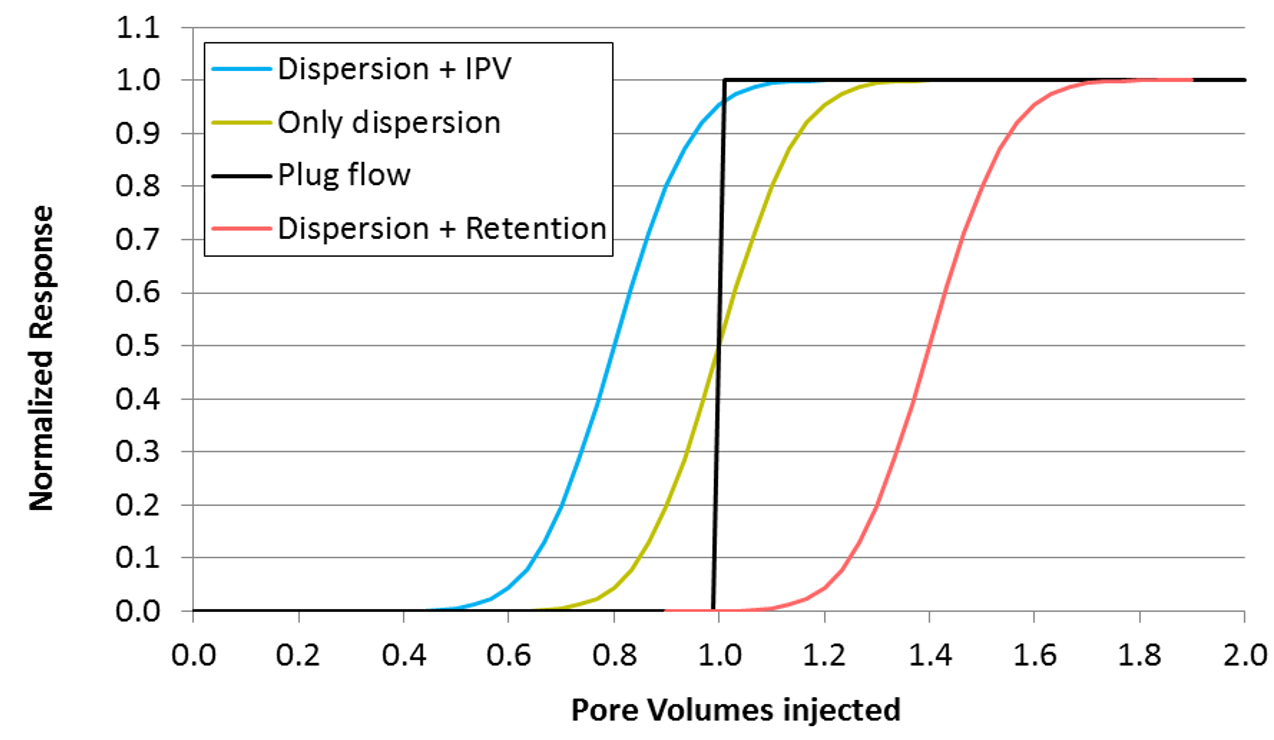
\includegraphics[width=\textwidth]{img/fig/ipvRet1.png}
    \caption{Effect of dispersion, inaccessible pore volume (IPV) and retention on relative responses.}
    \label{fig:ipvRet1} % 5.1
\end{figure}

In order to determine inaccessible pore volume of e.g., polymer, one can compare the production profiles of polymer and a tracer as a function of pore volumes injected. Figure \ref{fig:ipvRet2} illustrates such a comparison. The relative response of polymer is the ratio of measured effluent concentration to the injected concentration. The tracer should ideally have no IPV, i.e., the area below the tracer response should be equal to one. Changing the concentration in salt tracer will yield a close enough response. The area between the two responses determines the IPV.

\begin{figure}[h!]
    \centering
    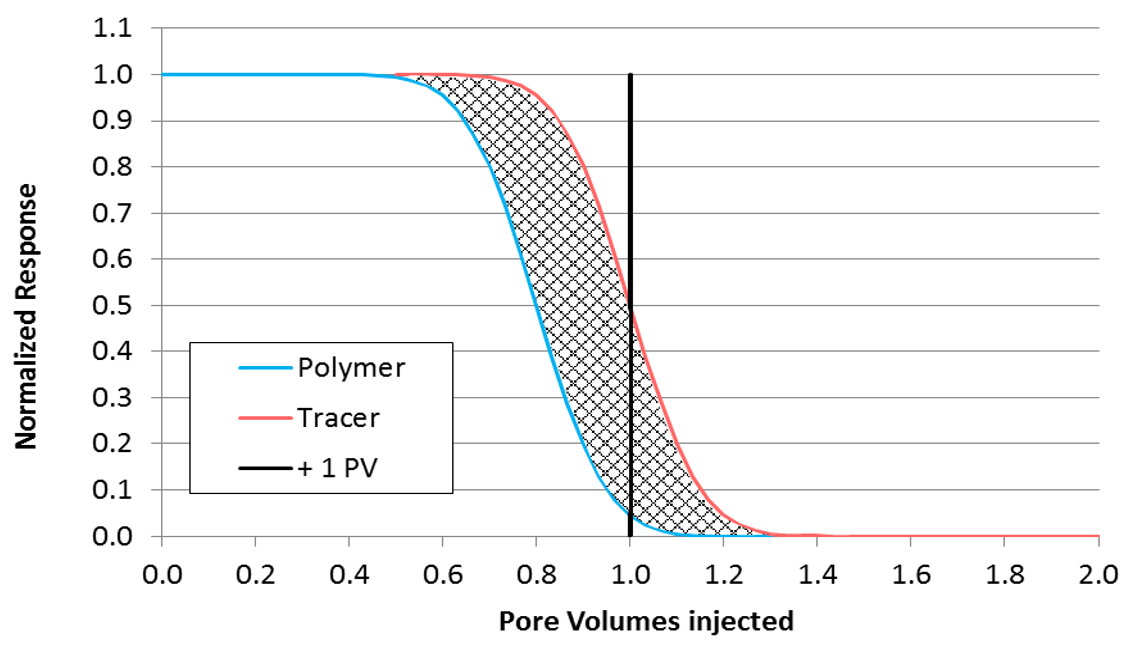
\includegraphics[width=\textwidth]{img/fig/ipvRet2.png}
    \caption{Effect of dispersion, inaccessible pore volume (IPV) and retention on relative responses.}
    \label{fig:ipvRet2} % 5.2
\end{figure}

Provided that the adsorption of polymer is irreversible and no mechanically entrapped polymer is released during water injection, the IPV will result in a response curve with an area under the curve of less than 1. Thus, IPV for polymer will be a positive value. However, if the system experiences desorption of the mechanically entrapped component, the area under the curve may become larger than the tracer area, resulting in a negative IPV indicating release of retained component. 

Total retention of a component in the rock depends on adsorption and mechanical entrapment. A multi-slug experiment can be used to quantify adsorption. Assuming that adsorption for the component under study were irreversible, all the adsorption happened in the first slug, i.e., no more adsorption took place during the second slug, and the magnitude of mechanical entrapment in both slugs were equal, one can compare the relative responses from the two slugs to find adsorption for the component. This is illustrated in Figure \ref{fig:ipvRet3}.

\begin{figure}[h!]
    \centering
    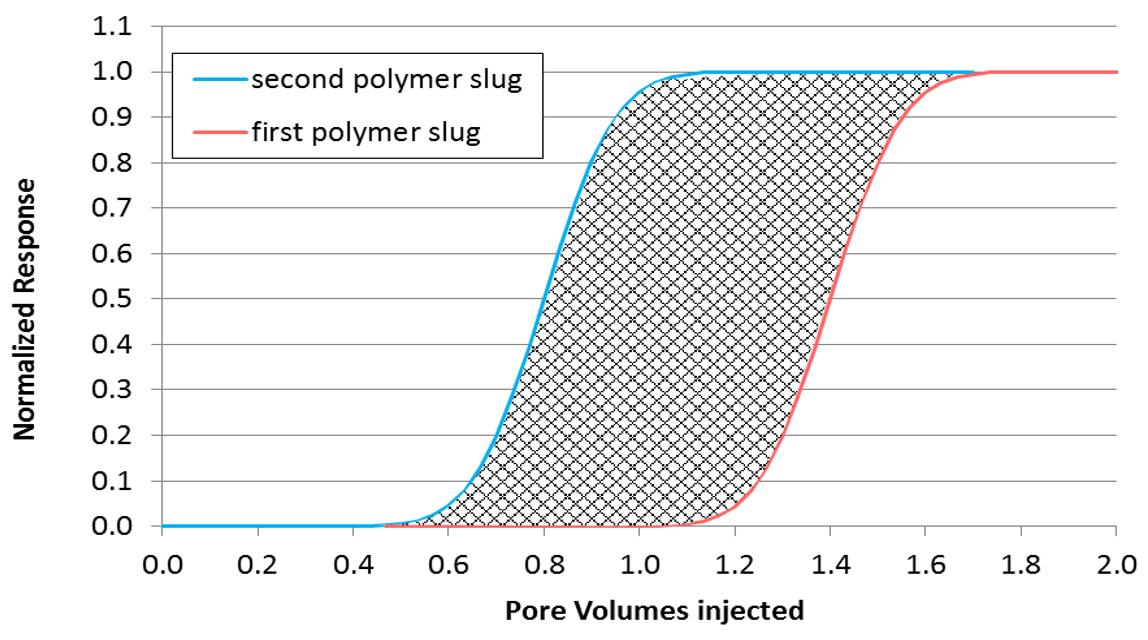
\includegraphics[width=\textwidth]{img/fig/ipvRet3.png}
    \caption{Effect of dispersion, inaccessible pore volume (IPV) and retention on relative responses.}
    \label{fig:ipvRet3} % 5.3
\end{figure}